\documentclass[a4paper,14pt]{article}
\usepackage[utf8]{inputenc}
\usepackage{verbatim}
\usepackage{lstautogobble}
\usepackage[french]{babel}
\usepackage[T1]{fontenc}
\usepackage{fancyvrb}
\usepackage{upquote}
\usepackage{fancybox}
\usepackage{pdfpages}
\usepackage[ left=1cm, right=1cm, top=2cm, bottom=2cm, heightrounded]{geometry}
\usepackage{fancyheadings} 
\lhead{}
\usepackage{fancyhdr}
\pagestyle{fancy}
\renewcommand{\headrulewidth}{2pt}
\fancyhead[C]{\LARGE{Propriété immobilière et comportements électoraux}}
\fancyhead[R]{}
\renewcommand{\footrulewidth}{2pt}
\fancyfoot[C]{} 
\fancyfoot[L]{BARRAU, DIEUDONNE, MAILLEFERT}
\fancyfoot[R]{\textbf{page \thepage}}
\usepackage{multirow}
\usepackage{array}
\usepackage{listings}
\usepackage{longtable}
\usepackage{amsmath,amssymb,amsfonts,graphicx,shorttoc,textpos,caption,here,titlesec}
\usepackage{verbatim,enumerate,hyperref,dsfont,fancyhdr,setspace,array}
\usepackage{eurosym}
\usepackage{titlesec}

\setlength{\textfloatsep}{0.1cm}
\usepackage{multirow}
\usepackage{url}
\urlstyle{sf}

\usepackage{float}
\usepackage[utf8]{inputenc}
\usepackage{multicol}
\newcommand{\squeezeup}{\vspace{-1cm}}
\titlespacing{\subsubsection}{0pt}{4pt}{4pt}
\setlength{\textfloatsep}{1cm}
\addto\captionsfrench{\def\tablename{Tableau}}
\usepackage{verbatim,enumerate,hyperref,dsfont,fancyhdr,setspace,array,csquotes}
\hypersetup{colorlinks=true,linkcolor=black, citecolor=black, urlcolor=black}
\usepackage[section]{placeins}
\linespread{1.1}\setlength{\columnsep}{25pt}

\usepackage[style=authoryear,citestyle=ext-authoryear,backend=biber,brackets]{biblatex} 
\DeclareOuterCiteDelims{parencite}{\bibopenbracket}{\bibclosebracket}

\usepackage[]{fncychap}
\usepackage{enumitem}
\newenvironment{itemize*}
{\begin{itemize}[leftmargin=*]
  \setlength{\itemsep}{0pt}
  \setlength{\parskip}{0pt}}
{\end{itemize}}

\title{Stat'app conflit politique}
\addbibresource{references.bib}



\begin{document}




\begin{titlepage}

\newcommand{\HRule}{\rule{\linewidth}{0.5mm}}

\center

% \textsc{\LARGE ENSAE}\\[0.5cm]

\includegraphics[scale=1.0]{ensae_logo_dev.png}\\[1cm]
\textsc{\Large Projet de statistiques appliquées}\\[0.5cm]

\HRule \\[0.4cm]
{ \huge \bfseries Propriété immobilière et comportements électoraux}\\[0.4cm]
\emph{\Large Note de synthèse de mi-parcours}\\[0.1cm]
\HRule \\[0.6cm]
\begin{center}
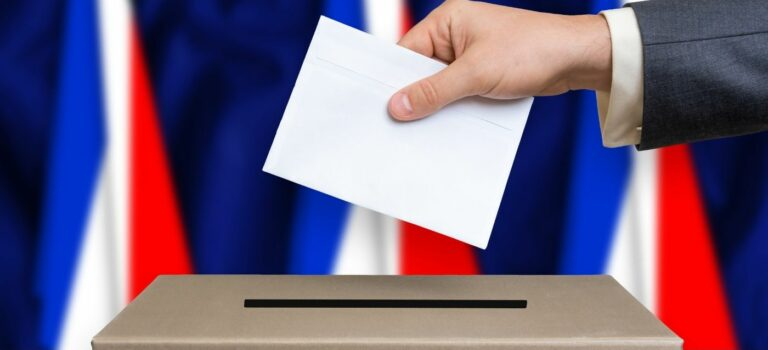
\includegraphics[scale=0.7]{Vote_image.jpg} 
\end{center}
\vspace{1cm}

\begin{minipage}{0.4\textwidth}
\begin{flushleft} \large
\emph{Auteurs}\\
Alexis \textsc{Barrau}\\
Maël \textsc{Dieudonné}\\
Swann \textsc{Maillefert}\\
\end{flushleft}
\end{minipage}\\[1cm]

\begin{minipage}{0.4\textwidth}
\begin{flushleft} \large
\emph{Encadrants}\\
Pauline \textsc{Mendras}\\
Gaston \textsc{Vermersch}\\
\end{flushleft}
\end{minipage}\\[1cm]

\begin{minipage}{0.4\textwidth}
\begin{flushleft} \large
\emph{Répertoire de travail}\\
\url{github.com/Alexis-Barrau/statappensae}\\
\end{flushleft}
\end{minipage}\\[1cm]


 ---------------------------------------------------------------------------------------\\[0.2cm]

{\large \today}\\[2cm]
\vfill

\end{titlepage}



\hspace{6mm} 


\begin{multicols}{2}

\section*{Introduction}
Le vote constitue un problème classique en sciences sociales depuis les travaux pionniers d'André Siegfried sur la géographie électorale \parencite{siegfried_tableau_1980}. Des analyses quantitatives, inaugurées aux États-Unis par Paul Lazarsfeld dans les années 1940 \parencite{lazarsfeld_peoples_2021}, ont isolé plusieurs grands déterminants du vote~: appartenance socioprofessionnelle, religion, âge, sexe, degré d'instruction, lieu de résidence, etc. Schématiquement, les catholiques et les indépendants votent à droite, les salariés votent à gauche, tandis que les jeunes, les chômeurs et les peu diplômés s'abstiennent \parencite{douillet_sociologie_2023}.


Le statut de propriétaire immobilier pourrait constituer un déterminant supplémentaire. Historiquement, l'accès à la propriété apparaît depuis au moins un siècle comme un moyen de stabiliser le vote des classes populaires, en l'arrachant aux forces réactionnaires ou révolutionnaires \parencite{michel_cause_2006}. Dès leur origine à la fin du \textsc{xix}\ieme ~siècle, les politiques du logement soutiennent l'accession à la propriété (lois Siegfried en 1894, Ribot en 1908, Loucheur en 1928, etc.). Ce mouvement s'est accéléré dans les années 1970, avec notamment la mise en place d'aides à l'accession à la propriété depuis 1977, dispositif prolongé en 1995 par le prêt à taux zéro, aboutissant à une forte croissance du taux de propriétaires, de 37~\% des ménages en 1960 à 58~\% en 2022 (Figure 1). Une dernière évolution notable, au tournant des années 1990 et 2000, concerne les prix du logement : alors qu'ils étaient restés alignés sur le coût de la vie depuis 1965, ils connaissent désormais une forte inflation dans les métropoles et les régions touristiques. Les dernières générations rencontrent ainsi des difficultés croissantes pour accéder à la propriété.

    \begin{figure}[H]
    \centering
         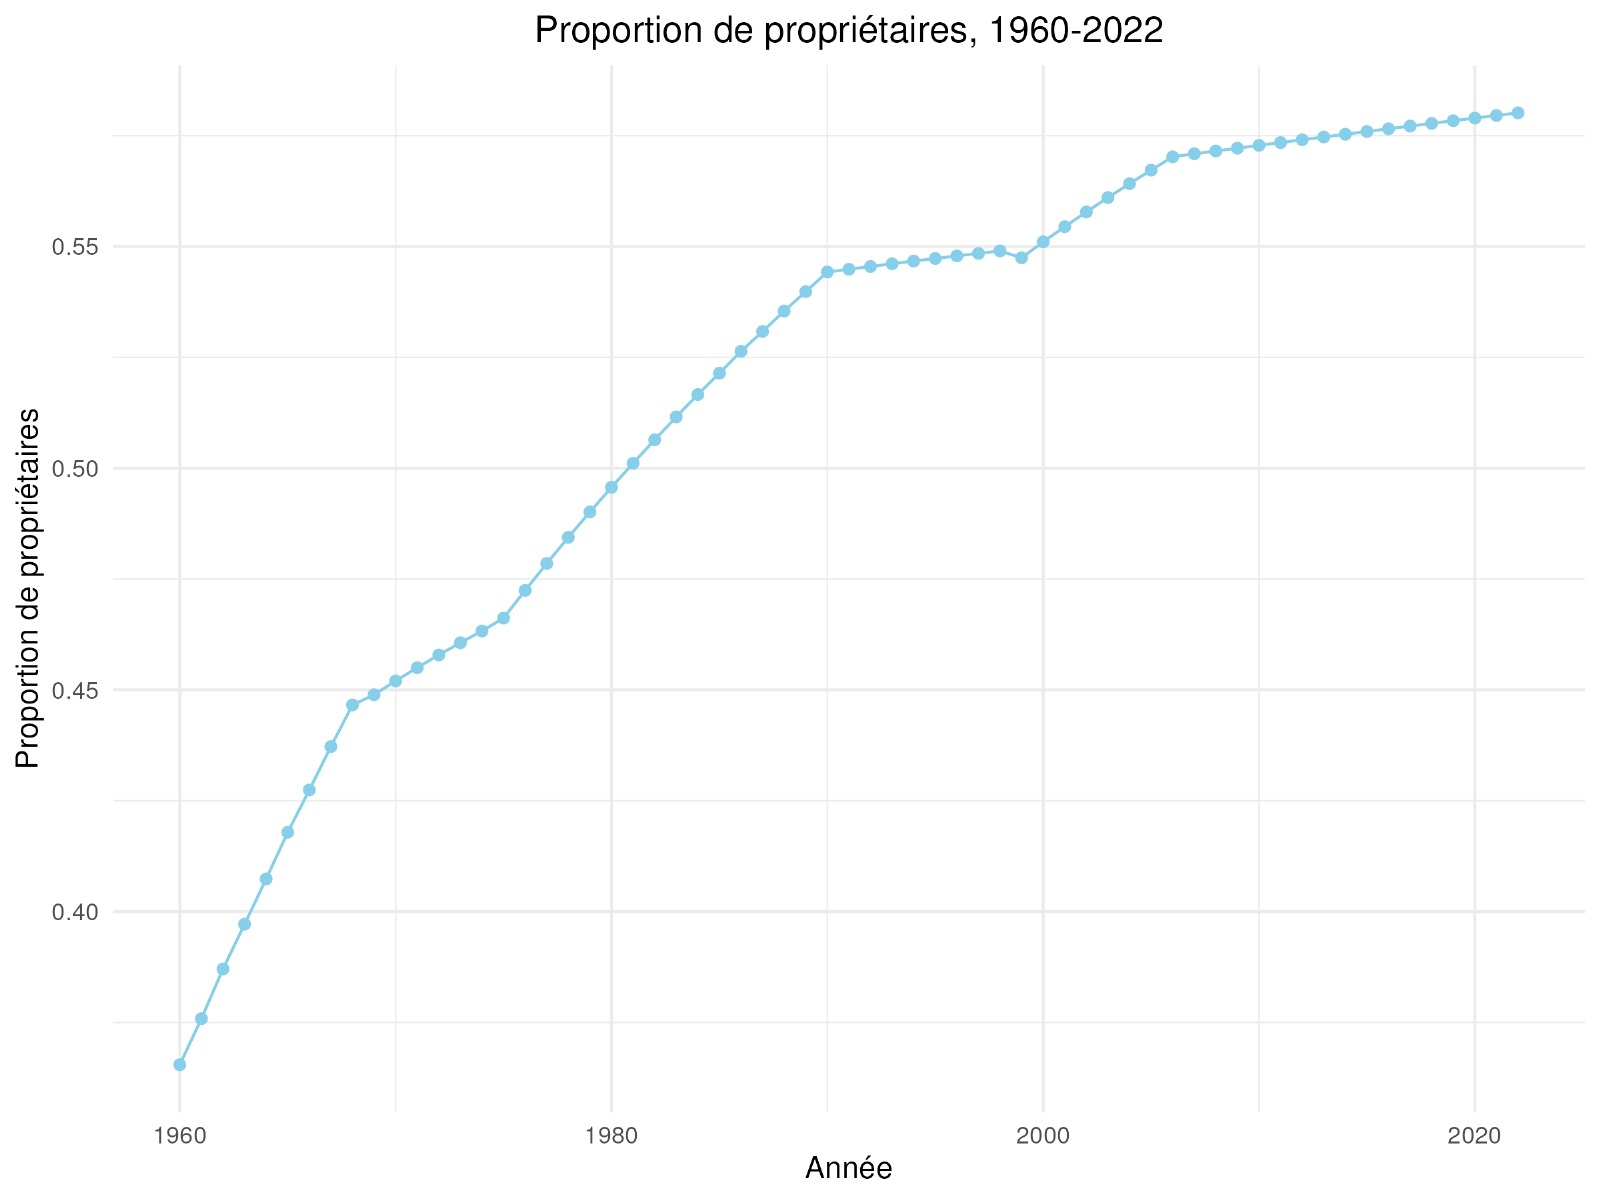
\includegraphics[width=8.5cm]{hist_tx_proprio.jpg}
         \caption{Proportion de propriétaires} 
         \source{\small \textit{Source : Données de Cagé et Piketty}}
    \end{figure}

Analysant les résultats des législatives de 1978, Capdevielle \textit{et al.} \parencite{capdevielle_france_1998} isolent une corrélation entre la détention d'un capital important et le vote à droite. L'hypothèse d'un effet spécifique du statut de propriétaire immobilier sur le vote a été particulièrement abordée dans le travail récent de Beckmann, Fulda et Kohl \parencite{beckmann_housing_2020} sur l'Allemagne. Ils identifient deux relations causales entre la propriété immobilière et le vote. Une relation d'intérêt («~vote économique~»)~: les propriétaires voteraient plus pour les partis conservateurs, ceux-ci protégeant davantage la propriété. Et une influence indirecte du mode de vie («~sociabilisation~»)~: l'accession à la propriété, s'effectuant dans des quartiers périurbains éloignés des infrastructures collectives, encouragerait une attitude davantage individualiste, plus cohérente avec un vote à droite. Les auteurs constatent que le statut de propriétaire influence le choix entre les partis conventionnels, c'est-à-dire entre la droite et la gauche du gouvernement, mais que ses effets s'estompent sur le vote protestataire. Ils observent également un embourgeoisement de l'électorat de gauche, qui compte un nombre croissant de propriétaires, ce qui conduit à un affaiblissement des effets de la propriété sur les pratiques de vote au cours du temps.


Le travail de Cagé et Piketty \parencite{cage_histoire_2023}, grâce à la constitution d'une base de données considérable, permet d'approcher cette question de façon différente. Ils cherchent à montrer l'importance de ce qu'ils appellent la «~classe géo-sociale\footnote{«~Inclut la question de la relation au territoire et aux ressources naturelles, aux moyens de transports et aux sources d'énergie, mais [...] doit être comprise de façon plus large dans ses dimensions socio-économiques~», en particulier les inégalités «~d'accès aux transferts et services sociaux~», de «~détention des moyens de production, de la hiérarchie des salaires et des revenus, de l'accès à la propriété et au logement, de justice sociale et fiscale~»}~» dans l'explication des comportements électoraux, au détriment notamment de critères que l'on pourrait qualifier de «~culturels~», en particulier depuis le milieu du \textsc{xx}\ieme ~siècle. 
Pour cela, ils procèdent à des analyses consistant principalement à comparer les résultats électoraux entre des quantiles de communes calculés relativement à une variable spécifique (revenu, diplôme...). Ils s'intéressent également à la capacité prédictive de l'appartenance géo-sociale, au travers de l'évolution temporelle du R² des régressions des résultats électoraux sur les variables correspondantes.
Dans ce cadre, l'accès à la propriété est bien prise en compte, mais assez peu étudiée indépendamment. Cagé et Piketty montrent néanmoins que depuis le milieu du \textsc{xx}\ieme ~siècle, l'écart de participation électorale s'est accru entre les communes contenant le plus de propriétaires et celles en contenant le moins. De même, ils constatent que les communes présentant les plus forts taux de propriétaires votent généralement plus à droite, et plus encore pour la droite dite «~nationale~». Ils expliquent notamment ce résultat par l'hostilité supposée d'une partie de la gauche envers la propriété privée, qui se manifesterait par une prédilection en faveur de politiques locatives.
\newline

L'objectif de ce projet de statistique appliquée est d'explorer davantage les effets du statut de propriétaire immobilier sur les comportements électoraux, à partir des données collectées par Cagé et Piketty. Leur équipe a constitué une base historique complète sur les élections nationales en France depuis deux siècles, enrichie de nombreuses données socio-démographiques par commune. Il s'agit de vérifier si l'on peut distinguer un effet spécifique du statut de propriétaire immobilier, indépendamment de caractéristiques éco-socio-démographiques.



\section*{Les données}
Le fonctionnement démocratique en France repose sur l'idée d'un vote de conviction, par lequel l'électeur exprimerait sa pleine souveraineté et individualité. Cela suppose, en particulier depuis la généralisation de l'isoloir au tournant des \textsc{xix}\ieme-\textsc{xx}\ieme ~siècles, le secret du vote \parencite{garrigou_les_1988}. Dès lors, l'étude de ce dernier est particulièrement difficile~: les données individuelles sont nécessairement déclaratives, sans garantie d'exhaustivité ni de correspondance avec les comportements réels, tandis que les données objectives, lorsqu'elles existent, sont nécessairement collectives, étant collectées au mieux à l'échelle des bureaux de vote.


Cagé et Piketty optent pour la seconde approche. Ils étudient les comportements électoraux à l'échelle le plus souvent communale, mais parfois aussi départementale ou cantonale, en croisant les données\footnote{Disponibles sous \url{https://unehistoireduconflitpolitique.fr/telecharger.html}} sur les phénomènes suivants~: résultats électoraux, population, géographie (typologie de commune), caractéristiques socio-démographiques (âge,  sexe, structure des ménages...), formation, diplômes, religion, catégorie socio-professionnelle, nationalité, statut migratoire, revenus, capital immobilier et terres agricoles et enfin d'autres données socio-économiques localisées (allocataires du RSA, crimes et délits ou contribuables ISF). Les sources mobilisées sont multiples (procès verbaux électoraux, recensement, archives nationales, données sur la taxation, DGFIP, CNAF...), détaillées dans l'annexe de leur ouvrage\footnote{https://conflit-politique-data.ams3.cdn.digitaloceanspaces.com/pdf/CagePiketty2023Annexes.pdf}. La variable qui nous intéresse plus particulièrement est la proportion de ménages propriétaires de leur résidence principale, disponible dans chaque commune à partir de 1960. L'information est collectée à partir des différents recensements puis interpolée de façon linéaire pour les années manquantes entre deux recensements\footnote{Années utilisées : 1962, 1968, 1975, 1982, 1990, 1999, 2006, 2021. Voir le dofile de recodage "doAnnexeB7proprietairescommunes" disponible sur le site compagnon du livre. Les auteurs n'ont pas utilisé les données du recensement de 2016, mais précisent que le taux national de propriétaires est resté très stable entre 2006 et 2021.}.


La constitution et l'utilisation d'une telle base de données soulève plusieurs difficultés théoriques (en plus des difficultés pratiques d'accès aux archives, de numérisation des données, etc) et notamment~: 
\newline   
\textbf{(1)} La catégorisation des territoires~: il est de plus en plus reconnu qu'ils exercent un effet spécifique sur les comportements électoraux, mais comment distinguer de façon univoque les villes des campagnes, les centres des banlieues, etc. ? Même pour la période actuelle, il n'y a pas d'accord des géographes sur une typologie des territoires, et l'Insee utilise plutôt des catégories fonctionnelles.
Cagé et Piketty proposent finalement une quadripartition des communes en villages, bourgs, banlieues et métropoles, en appliquant rétrospectivement la nomenclature 2022 des unités urbaines jusqu'en 1793. Cette approche nous semble contestable, et nous préférons ne pas réutiliser la classification associée.
\newline
\textbf{(2)} La classification politique des candidats, dans un espace politique complexe et dynamique~: les auteurs rappellent ainsi que si certains pays connaissent une assez grande stabilité dans le temps de leurs structures partisanes (Royaume-Uni, États-Unis), ce n'est pas le cas de la France pour laquelle ils dénombrent une multiplicité de courants au cours du temps, alors que les luttes politiques ne sont, de plus, jamais réductibles à une simple opposition droite-gauche. Il est néanmoins indispensable, dès lors que l'on cherche à réaliser un traitement statistique, en particulier diachronique, d'opérer des regroupements. Si nous pourrons être amenés à mobiliser les regroupements opérés par Cagé et Piketty, nous pourrons aussi mobiliser les nôtres à partir des données brutes disponibles dans la base, qu'il s'agira d'expliciter et de justifier. 


Par ailleurs, il nous semble important ici de mentionner les difficultés inhérentes à la manipulation de bases de données de cette ampleur, fractionnées dans de multiples bases (une par élection et une pour chaque dimension des variables explicatives) qu'il a fallu regrouper et nettoyer afin de les rendre utilisables pour ce projet de statistiques appliquées. Ce travail\footnote{Documenté dans le code disponible sur notre dépôt git.} nous a ainsi beaucoup occupé dans la première partie du projet.

\section*{Méthodes}
Nous avons fait le choix de nous intéresser exclusivement aux élections présidentielles ayant eu lieu au suffrage universel sous la \textsc{V}\ieme République, c'est-à-dire depuis 1965. Cette restriction présente en effet plusieurs avantages importants. Tout d'abord, les élections présidentielles sont nationales, avec des candidats clairement identifiés, ce qui limite les problèmes de classification politique évoqués \textit{supra} et renforce la lisibilité de leurs enjeux, que l'on peut supposer homogènes sur l'ensemble du territoire. Elles ont aussi l'avantage d'avoir conservé un mode de scrutin uniforme au cours du temps, facilitant ainsi les comparaisons entre elles. Enfin, et de manière plus prosaïque, elles coïncident avec la disponibilité d'informations provenant de sources statistiques fiables. La proportion de ménages propriétaires de leur résidence principale, en particulier, n'est disponible qu'à partir de 1960. 

Nous avons choisi, en première analyse, de régler les difficultés précédentes en nous limitant à l'élection présidentielle de 1981, en nous passant donc de la dimension temporelle de nos données. Les candidats sont ainsi peu nombreux et faciles à positionner politiquement. Les analyses ont principalement été effectuées en R\footnote{Le code est intégralement disponible sur notre dépôt git.}.
\newline
Nous nous intéressons notamment aux variables suivantes~: 

\end{multicols}

\begin{center}
\begin{tabular}{|c||c|c|c||c|}
\hline
\textbf{Variables} & \textbf{1\ier quartile} & \textbf{Médiane} & \textbf{3\ieme quartile} & \textbf{pct NA} \\ 
\hline
participation & 0.805 & 0.842 & 0.873 & 0.63 \\
\hline
participation T2 & 0.864 & 0.891 & 0.915 & 0.44 \\
\hline
ratio vote gauche//droite & 0.391 & 0.484 & 0.566 & 0.63 \\
\hline
ratio vote gauche//droite T2 & 0.413 & 0.503 & 0.583 & 0.44 \\
\hline
part de propriétaires & 0.628 & 0.728 & 0.812 & 0.23 \\
\hline
\end{tabular}
\end{center}
\begin{multicols}{2}
Les effets de biais de sélection seront pris en compte par l'ajout de multiples variables de contrôle~: la répartition par tranche d'âge, la répartition par niveau de dipôme (sans diplôme, baccalauréat et enseignement supérieur), la religiosité, la répartition par catégorie socio-professionnelle, la proportion d'étrangers, des indicatrices départementales et enfin le revenu moyen. Toutefois, comme en témoigne le corrélogramme ci-dessous, toutes nos variables sont plus ou moins corrélées entre elles, ce qui va jouer sur la variance des estimateurs et donc sur les résultats de significativité, ainsi que sur le biais de variables omises.

\begin{figure}[H]
    \centering
         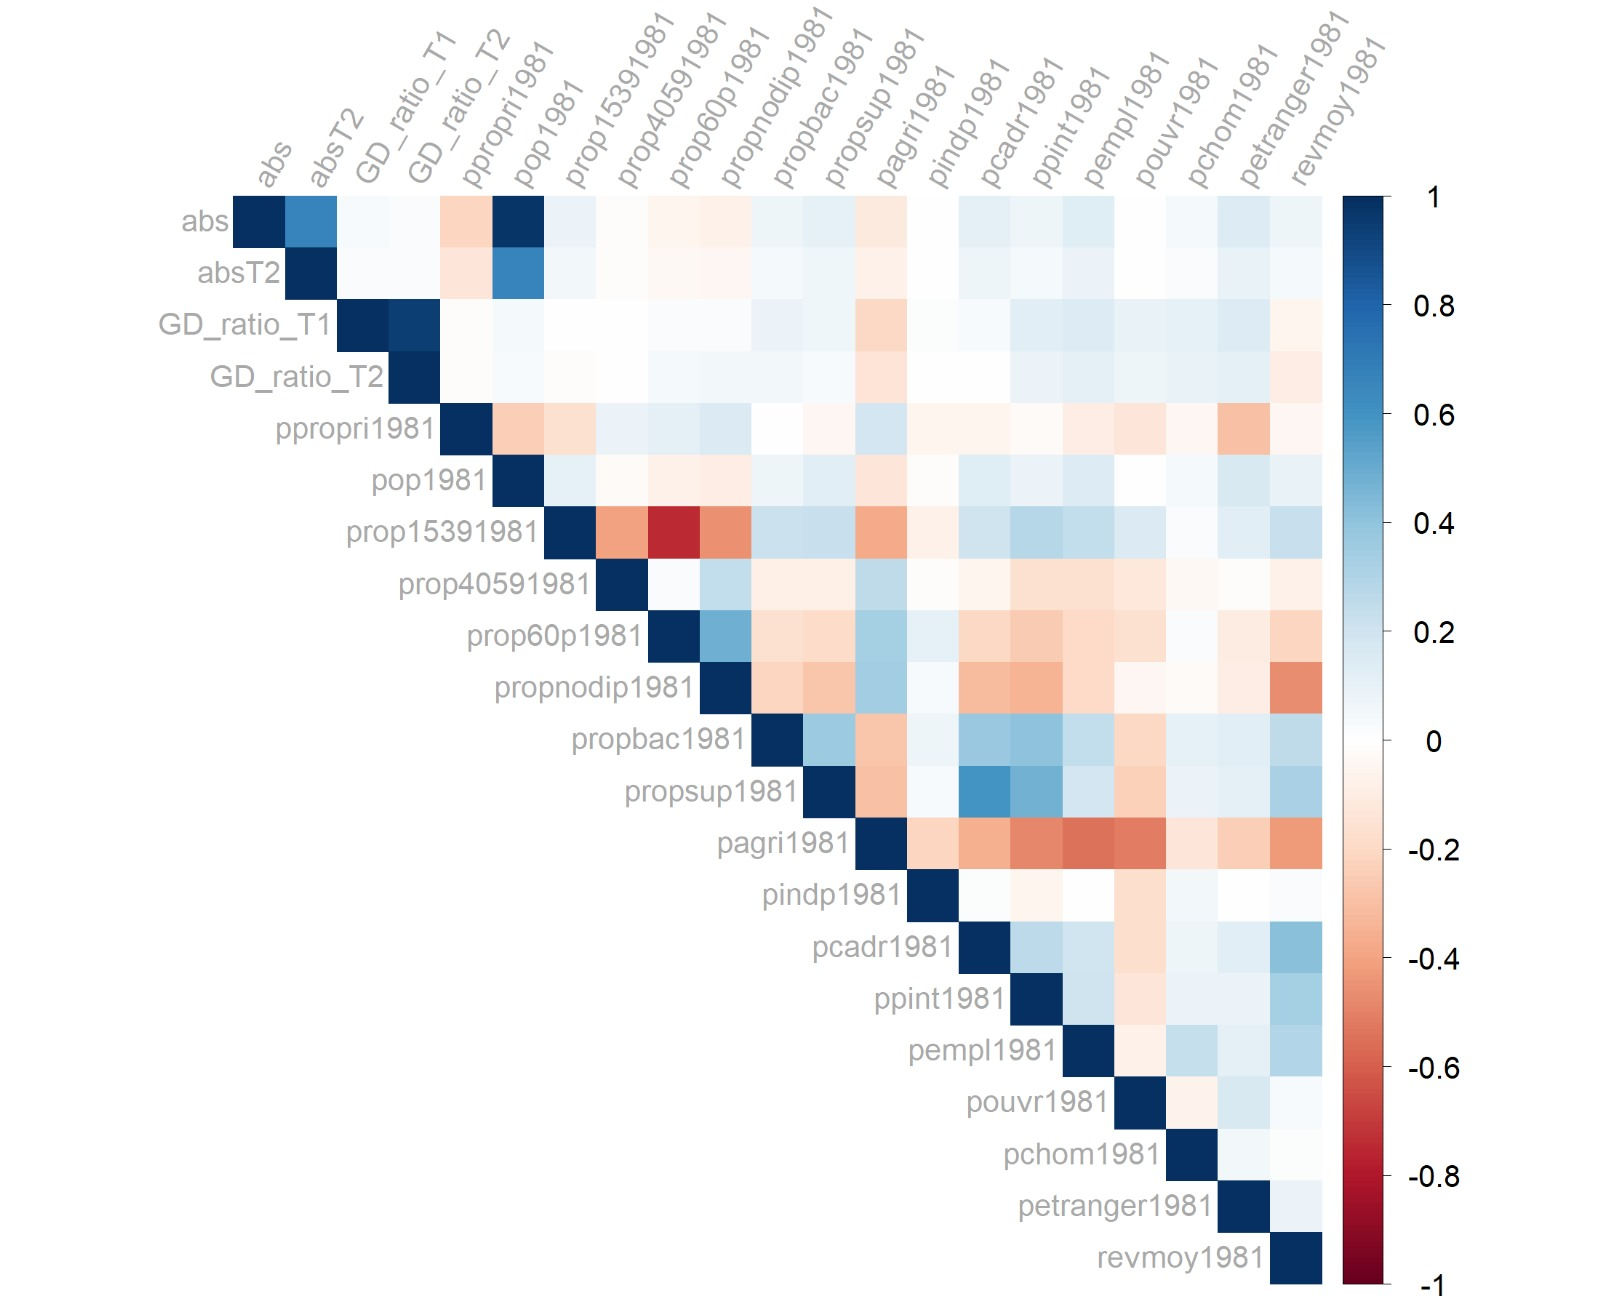
\includegraphics[width=8.5cm]{correlogramme.jpg}
         \caption{Corrélogramme de nos variables d'intérêt} 
         \source{\small \textit{Source : Données de Cagé et Piketty}}
    \end{figure}
    
Les régressions naïves du taux de participation et de la part de votes pour la gauche sur le taux de propriétaires et les variables de contrôles mettent en avant un effet significatif, de signe attendu, mais assez fortement sujet au biais de variables omises avec une grande variabilité du coefficient en fonction des ajouts (du fait des corrélations non négligeables entre nos variables). On retrouve également certains résultats avancés dans la littérature (influence du niveau de diplômes, de la part d'étrangers...). Notamment en raison du biais écologique, il n'est pas possible en l'état d'identifier un effet causal du taux de propriétaire.



\section*{Perspectives}
Nous avons commencé par partitionner l'espace politique selon un clivage bi-partisan gauche-droite, mais prévoyons d'expérimenter d'autres partitions afin de capter plusieurs dimensions des comportements électoraux : un ratio droite/gauche capturerait plutôt les enjeux économiques, un ratio centre/extrêmes le degré d'adhésion au système politique et un ratio libéralisme culturel/conservatisme moral permettrait de distinguer les enjeux économiques des enjeux sociétaux, etc.

Le traitement de la participation électorale constitue un autre problème classique. Elle est d'ordinaire analysée séparément des suffrages exprimés, ce qui engage une représentation forte des comportements politiques (avec des électeurs choisissant d'abord de voter, puis pour qui voter, comme si leur participation était indépendant de leur orientation politique et de l'offre partisane à chaque élection). Nous souhaitons explorer d'autres approches. La solution d'un modèle multinomial semble impraticable : elle impliquerait de reconstruire les données individuelles de millions d'individus pour une quinzaine de variables de contrôles, soulevant de redoutables problèmes de cohérence. Nous allons explorer des modèles de réduction de dimension avec projection de variables supplémentaires pour apporter des éléments d'analyse.


Concernant l'effet causal, nous introduirons dans un second temps la dimension temporelle à travers des modèles de panel pour modéliser une hétérogénéité non observée et ainsi réduire le biais de sélection. Nous considérerons un modèle à effets individuels inobservés $y_{it} = \theta_{t} + x_{it}\beta + c_{i}  + u_{it}$ avec $c_{i}$ les caractéristiques inobservées. Nos variables explicatives ne permettant pas de pouvoir raisonnablement supposer que $cov(c_{i}, x_{it}) = 0$, une modélisation à effets fixes sera appliquée. Il nous faudra dès lors travailler en différences premières $y_{i,t} - y_{i,t-1} = \alpha_{t} + (x_{i,t} - x_{i,t-1})\beta + (u_{i,t} - u_{i,t-1})$ ou en fluctuations 
$y_{i,t} - \Bar{y_{i}} = \alpha_{t} + (x_{i,t} - \Bar{x_{i}})\beta + (u_{i,t} - \Bar{u_{i}})$.

Pour terminer, relevons quelques limites de l'approche que nous envisageons. L'identification d'effets proprement causaux de la propriété sur les pratiques électorales semble \textit{a priori} difficile. En effet, aux effets de sélection classiques (différences d'âge, de revenus et de diplômes entre propriétaires et locataires) s'ajoute un problème de simultanéité, où la propriété et les pratiques de vote se déterminent mutuellement, comme l'illustrent les cartes suivantes.
\end{multicols}
\begin{figure}[H]
    \centering
    \begin{minipage}[t]{8.5cm}
         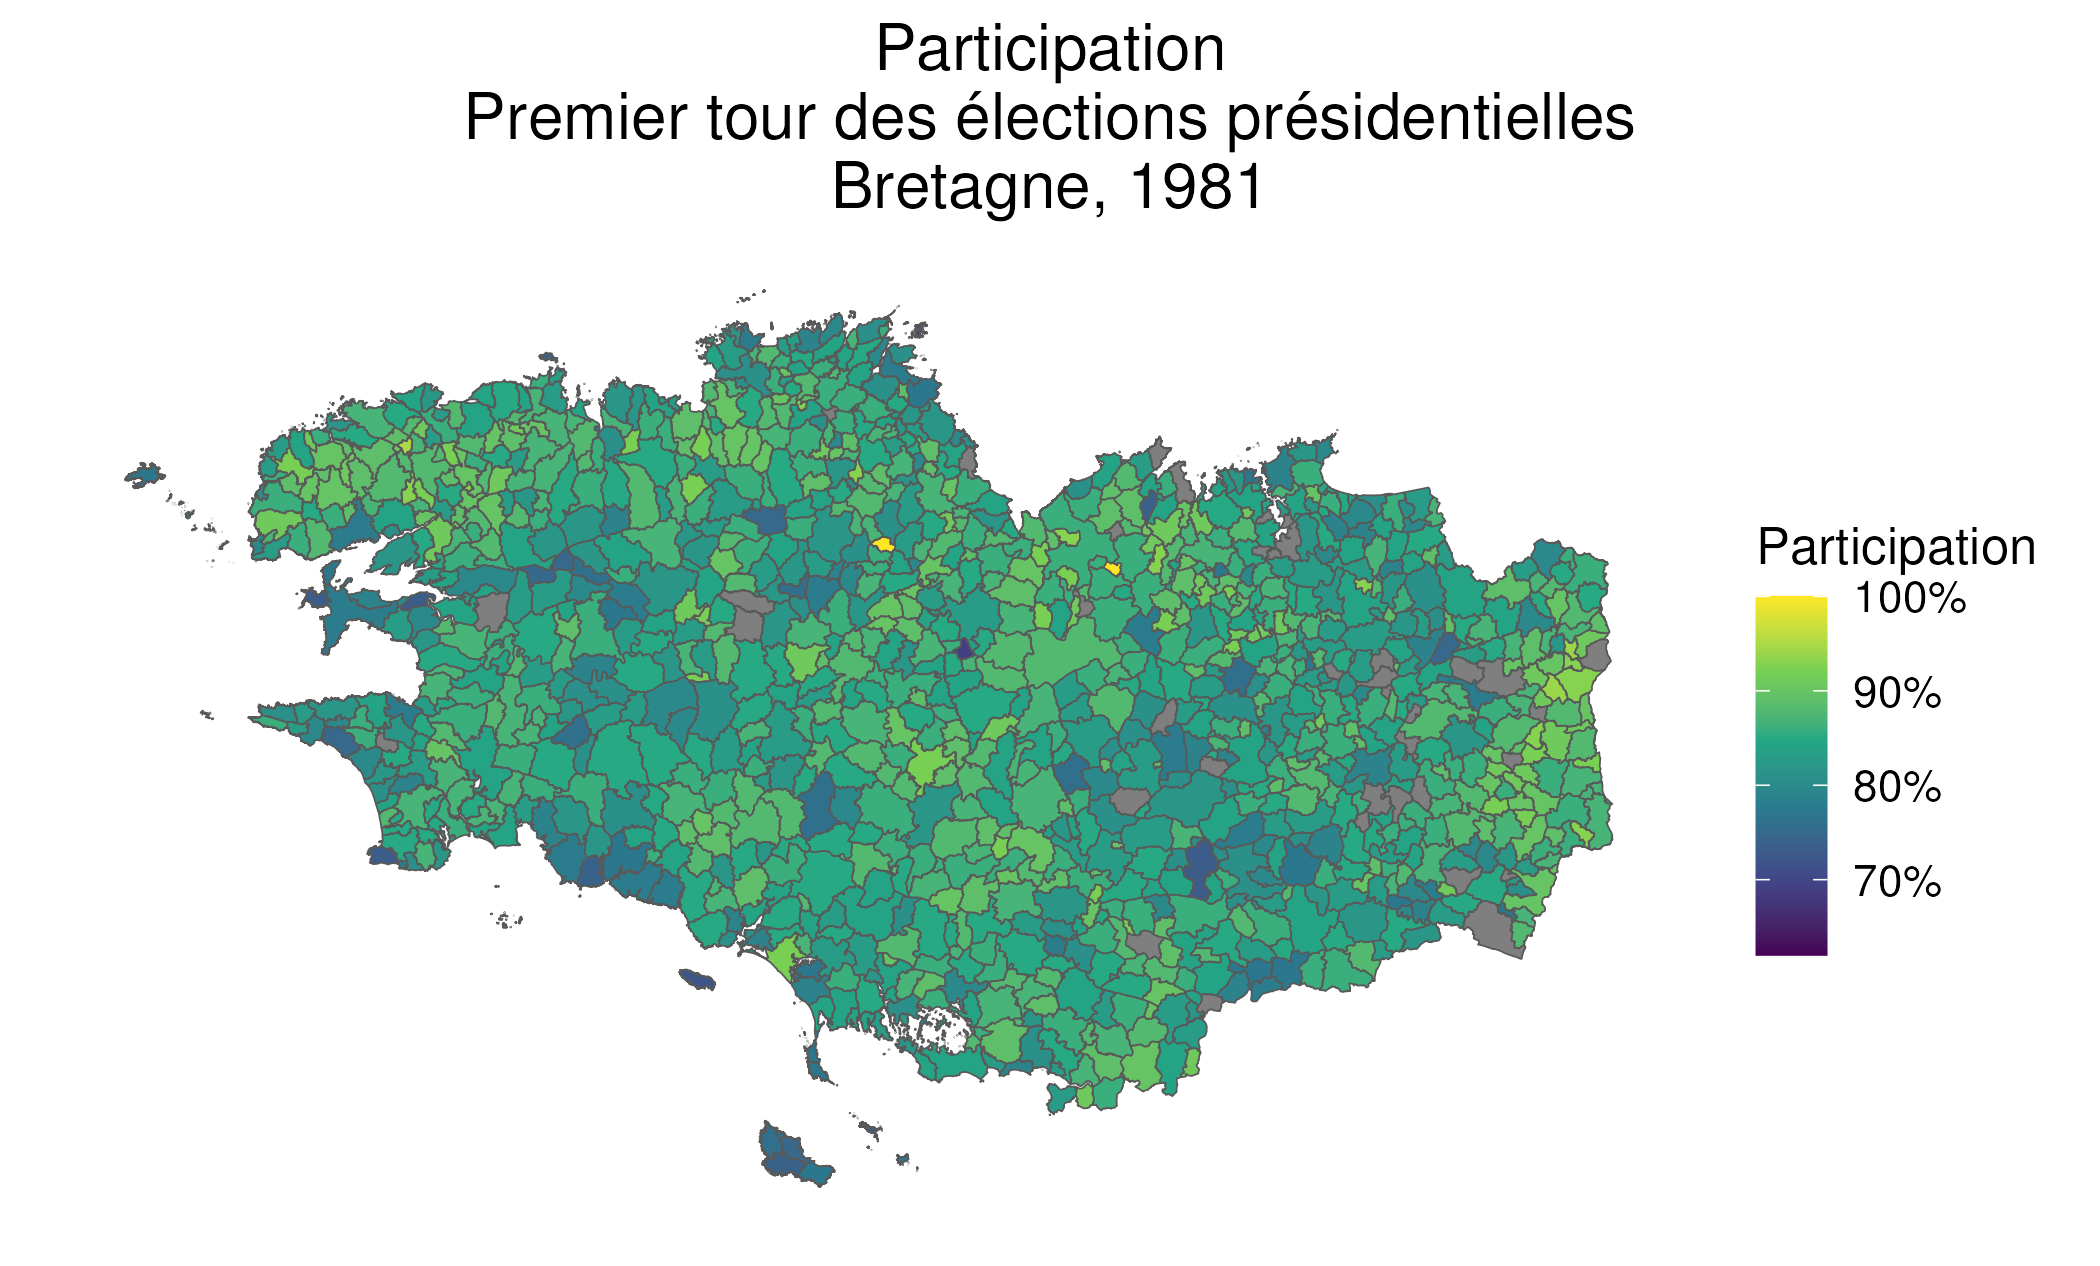
\includegraphics[width=8.5cm]{part_1981_Bre.png}
    \end{minipage}
    \begin{minipage}[t]{8.5cm}
        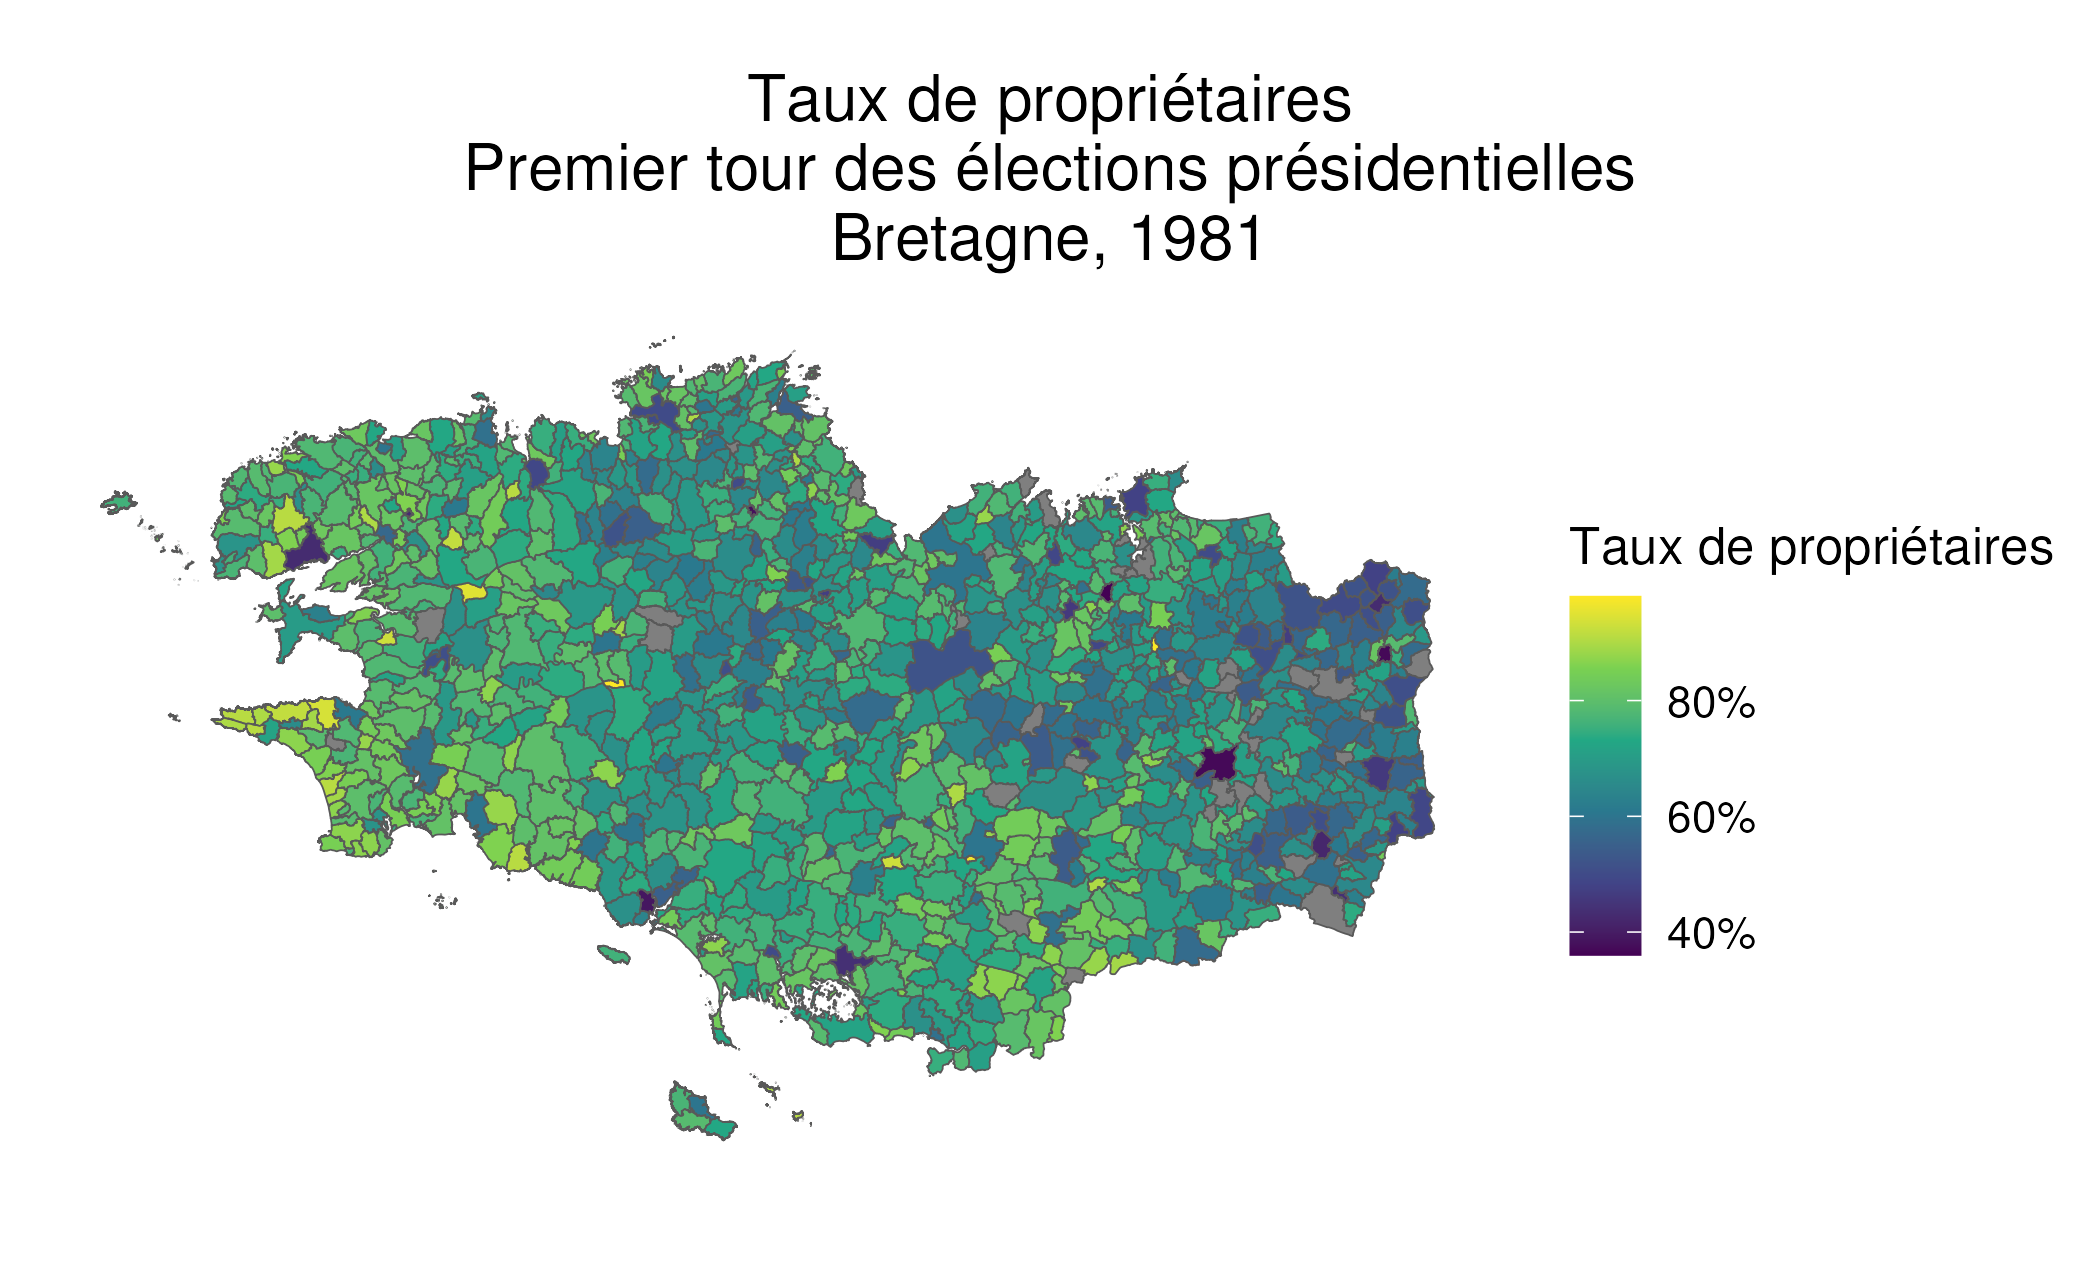
\includegraphics[width=8.5cm]{ppropri_1981_Bre.png}
    \end{minipage}
\end{figure}
\begin{multicols}{2}
 Un autre problème est l'identification du moment où la propriété exerce une influence (incubation et anticipation), sur lequel la profondeur historique des données disponibles pourrait apporter des éléments d'analyse. 
 
 Plus encore, la démarche que nous proposons se heurte au problème classique du «~biais écologique~» (ou encore «~biais d'inférence écologique~»). En effet, dès lors que l'on traite de données agrégées géographiquement, les comportements individuels sont inaccessibles, ce qui impose une grande prudence dans l'interprétation. Cagé et Piketty proposent l'exemple suivant~: si les communes riches ont un taux de participation plus élevé que les communes pauvres, il est impossible d'en conclure que les électeurs riches s'abstiennent moins que les électeurs pauvres, car rien ne prouve que ce soient eux qui votent davantage dans les communes riches. Ce problème a été discuté théoriquement, \textit{cf} King \parencite{king_solution_1997} pour une synthèse récente. Nous sommes néanmoins convaincu, suivant en cela les préconisations par exemple de Gombin et Mayance \parencite{gombin_analyse_2010}, que l'approche par données agrégées peut s'avérer fructueuse dès lors qu'elle s'accompagne de précautions interprétatives et de recoupement avec d'autres sources (analyses théoriques ou analyses reposant sur des données individuelles lorsque disponibles).



\end{multicols}
\printbibliography
\end{document}